\documentclass[12pt,a4paper]{article}

%!TEX program = pdflatex

% =============================================================================
% 1. PHÔNG CHỮ & NGÔN NGỮ (Hỗ trợ Tiếng Việt)
% =============================================================================
\usepackage[utf8]{inputenc}
\usepackage[T5]{fontenc}
\usepackage[vietnamese]{babel}

% =============================================================================
% 2. BỐ CỤC TRANG (LAYOUT)
% =============================================================================
\usepackage[margin=2.5cm]{geometry}
\usepackage{setspace}
\onehalfspacing

% =============================================================================
% 3. ĐỒ HỌA & BIỂU ĐỒ (TikZ & DFD Styles)
% =============================================================================
\usepackage{graphicx}
\usepackage{tikz}
\usetikzlibrary{arrows.meta, positioning, shapes.geometric}

\tikzset{
    process/.style={ellipse, draw, minimum width=3cm, minimum height=1.5cm, align=center},
    entity/.style={rectangle, draw, minimum width=2.5cm, minimum height=1cm, align=center},
    datastore/.style={
        draw=none, align=center, minimum width=3cm,
        append after command={
            [shorten <= -0.2cm, shorten >= -0.2cm]
            (\tikzlastnode.north west) edge (\tikzlastnode.north east)
            (\tikzlastnode.south west) edge (\tikzlastnode.south east)
        }
    },
    arrow/.style={-Stealth, thick}
}

% =============================================================================
% 4. BẢNG BIỂU & DANH SÁCH
% =============================================================================
\usepackage{array}
\usepackage{booktabs}
\usepackage{multirow}
\usepackage{longtable}
\usepackage{float}
\usepackage{enumitem}
\usepackage{tabularx}
\usepackage{makecell}
\usepackage{colortbl}

% =============================================================================
% 5. TIỆN ÍCH VĂN BẢN & LIÊN KẾT
% =============================================================================
\usepackage{xcolor}
\usepackage{titlesec}
\usepackage{tocloft}
\usepackage{xurl}
\usepackage{seqsplit}
\usepackage{hyperref}

\hypersetup{
    colorlinks=false,
    hidelinks,
    pdftitle={Mô hình hóa yêu cầu chức năng},
    pdfauthor={Tên của bạn}
}

% =============================================================================
% 6. ĐỊNH DẠNG ĐOẠN VĂN & ĐÁNH SỐ MỤC
% =============================================================================
\setlength{\parindent}{0pt}
\setlength{\parskip}{6pt}
\setcounter{secnumdepth}{3}

\renewcommand{\thesection}{\Roman{section}}
\renewcommand{\thesubsection}{\arabic{subsection}}
\renewcommand{\thesubsubsection}{\thesubsection.\arabic{subsubsection}}

\titleformat{\section}{\large\bfseries}{\thesection.}{0.5em}{}
\titleformat{\subsection}{\normalsize\bfseries}{\thesubsection.}{0.5em}{}
\titleformat{\subsubsection}{\normalsize\itshape\bfseries}{\thesubsubsection.}{0.5em}{}

\titleformat{\paragraph}[block]{\normalsize\bfseries}{}{0pt}{}
\titlespacing*{\paragraph}{0pt}{6pt}{0pt}

% =============================================================================
% 7. MỤC LỤC (TOC)
% =============================================================================
\renewcommand{\cftsecaftersnum}{.}
\renewcommand{\cftsubsecaftersnum}{.}
\renewcommand{\cftsubsubsecaftersnum}{.}

% =============================================================================
% 8. CUSTOM COMMANDS & COLUMN TYPES
% =============================================================================
\newcolumntype{C}[1]{>{\centering\arraybackslash}p{#1}}
\newcolumntype{L}[1]{>{\raggedright\arraybackslash}p{#1}}
\newcolumntype{Y}{>{\raggedright\arraybackslash}X}
\newcommand{\subsubsubsection}[1]{\paragraph{#1}}
\newcommand{\tablesetup}{\small\setlength{\tabcolsep}{3pt}\renewcommand{\arraystretch}{1.2}}
\newcommand{\code}[1]{{\ttfamily\seqsplit{#1}}}
\newcommand{\seqpdf}[1]{%
\IfFileExists{#1}{%
    \includegraphics[page=1,width=1.05\textwidth,height=0.95\textheight,keepaspectratio]{#1}%
}{%
    \fbox{%
        \parbox[c][0.28\textheight][c]{0.9\textwidth}{%
            \centering
            Chưa tìm thấy file \texttt{#1}.\\[4pt]
            Hãy upload đúng file PDF này lên Overleaf.
        }%
    }%
}%
}

\begin{document}

\section{Mô hình hóa yêu cầu chức năng}

Phần này trình bày mô hình hóa yêu cầu chức năng của hệ thống TMS. Các sơ đồ
tập trung vào nghiệp vụ, luồng dữ liệu và tương tác giữa người dùng với hệ
thống. Phần này không đi sâu vào chi tiết cài đặt hay cấu trúc mã nguồn.

\subsection{Tác nhân và sơ đồ use case tổng quan}

Các tác nhân chính của hệ thống gồm Giáo viên, Quản trị viên và Học sinh. Bên
cạnh đó, Discord và Codeforces là các hệ thống ngoài đóng vai trò tác nhân hỗ
trợ. Discord hỗ trợ các chức năng xác thực, thiết lập guild, gửi thông báo và
điểm danh voice. Codeforces hỗ trợ dữ liệu Gym và bảng xếp hạng.

\begin{figure}[H]
    \centering
    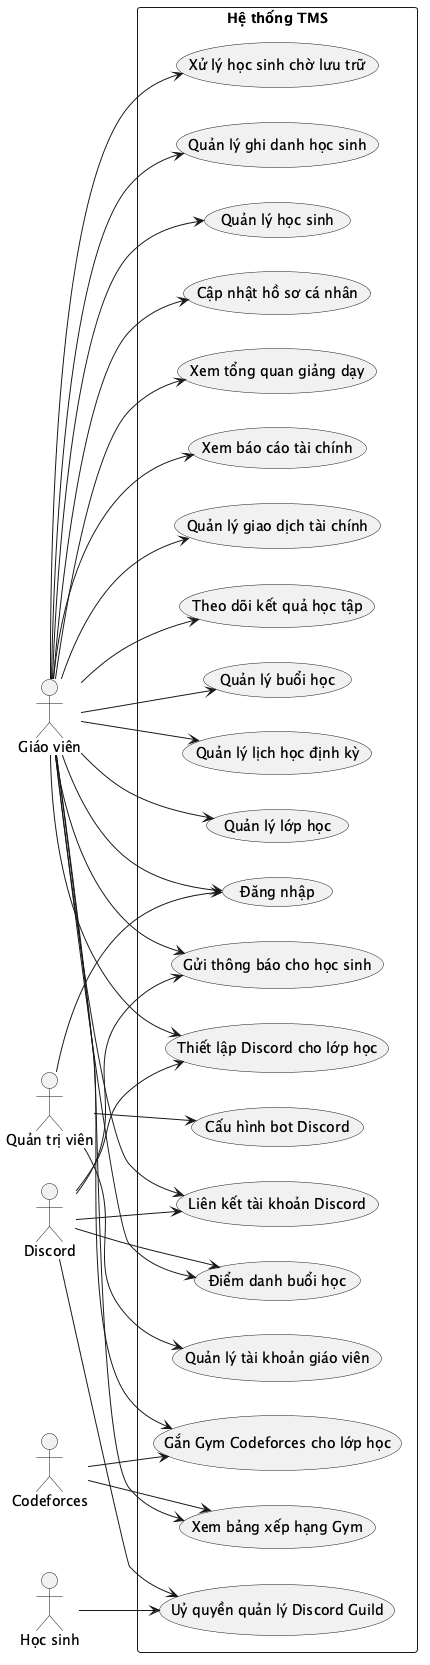
\includegraphics[width=0.95\textwidth,height=0.72\textheight,keepaspectratio]{diagrams/use-case-overview.png}
    \caption{Sơ đồ use case tổng quan}
\end{figure}

\subsection{Danh sách use case}

\begin{longtable}{L{3.2cm} L{11cm}}
\toprule
\textbf{Tác nhân} & \textbf{Use case} \\
\midrule
\endhead
Giáo viên & Đăng nhập; Xem tổng quan giảng dạy; Cập nhật hồ sơ cá nhân; Liên kết tài khoản Discord; Quản lý học sinh; Quản lý ghi danh học sinh; Xử lý học sinh chờ lưu trữ; Quản lý lớp học; Quản lý lịch học định kỳ; Quản lý buổi học; Điểm danh buổi học; Theo dõi kết quả học tập; Quản lý giao dịch tài chính; Xem báo cáo tài chính; Thiết lập Discord cho lớp học; Gửi thông báo cho học sinh; Gắn Gym Codeforces cho lớp học; Xem bảng xếp hạng Gym. \\
Quản trị viên & Đăng nhập; Quản lý tài khoản giáo viên; Cấu hình bot Discord. \\
Học sinh & Uỷ quyền quản lý Discord Guild. \\
Discord & Tác nhân hỗ trợ cho các use case liên quan đến Discord OAuth, guild, channel, tin nhắn và voice state. \\
Codeforces & Tác nhân hỗ trợ cho các use case liên quan đến Gym và bảng xếp hạng. \\
\bottomrule
\end{longtable}

\subsection{Quy ước mô tả chức năng}

Mỗi chức năng được mô tả bằng tóm tắt, tác nhân, tiền điều kiện, dòng sự kiện
chính, dòng sự kiện phụ, hậu điều kiện, sơ đồ luồng dữ liệu và sơ đồ hoạt động.
DFD được sử dụng cho mọi chức năng để mô tả dữ liệu đi từ tác nhân ngoài vào
khối xử lý, dữ liệu được đọc/ghi ở kho dữ liệu và dữ liệu đầu ra trả về cho tác
nhân. Activity diagram được đặt riêng trong từng use case để mô tả luồng xử lý
của use case đó. Các sequence diagram hoặc collaboration diagram chỉ được bổ
sung trong chính use case liên quan khi luồng đủ phức tạp.

\subsection{Mô tả chi tiết các use case}


\subsubsection{Đăng nhập}

\textbf{Tóm tắt:} Cho phép người dùng hợp lệ truy cập hệ thống theo đúng vai trò được cấp.

\textbf{Tác nhân:} Giáo viên, Quản trị viên

\textbf{Tiền điều kiện}
\begin{itemize}[leftmargin=*]
    \item Người dùng có tài khoản trong hệ thống.
    \item Hệ thống đang kết nối được với cơ sở dữ liệu.
\end{itemize}

\textbf{Dòng sự kiện chính}
\begin{enumerate}[leftmargin=*]
    \item Người dùng mở màn hình đăng nhập.
    \item Người dùng nhập tên đăng nhập và mật khẩu.
    \item Hệ thống kiểm tra thông tin đăng nhập.
    \item Hệ thống kiểm tra trạng thái và vai trò tài khoản.
    \item Hệ thống cấp phiên đăng nhập và chuyển người dùng vào màn hình chính.
\end{enumerate}

\textbf{Dòng sự kiện phụ}
\begin{itemize}[leftmargin=*]
    \item Nếu thiếu thông tin đăng nhập, hệ thống yêu cầu nhập đầy đủ.
    \item Nếu thông tin đăng nhập không chính xác, hệ thống thông báo lỗi.
    \item Nếu tài khoản không còn hoạt động, hệ thống từ chối đăng nhập.
\end{itemize}

\textbf{Hậu điều kiện}
\begin{itemize}[leftmargin=*]
    \item Người dùng đăng nhập thành công và sử dụng được các chức năng theo quyền hạn.
\end{itemize}

\textbf{Sơ đồ luồng dữ liệu}

\begin{figure}[H]
    \centering
    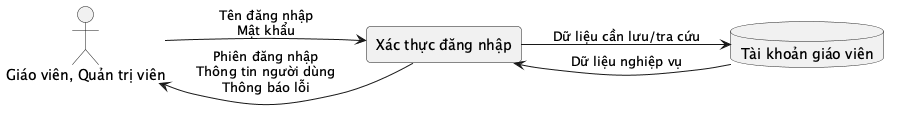
\includegraphics[width=0.95\textwidth,height=0.72\textheight,keepaspectratio]{diagrams/dfd-dang-nhap.png}
    \caption{Sơ đồ luồng dữ liệu: undefined}
\end{figure}

\textbf{Sơ đồ hoạt động}

\begin{figure}[H]
    \centering
    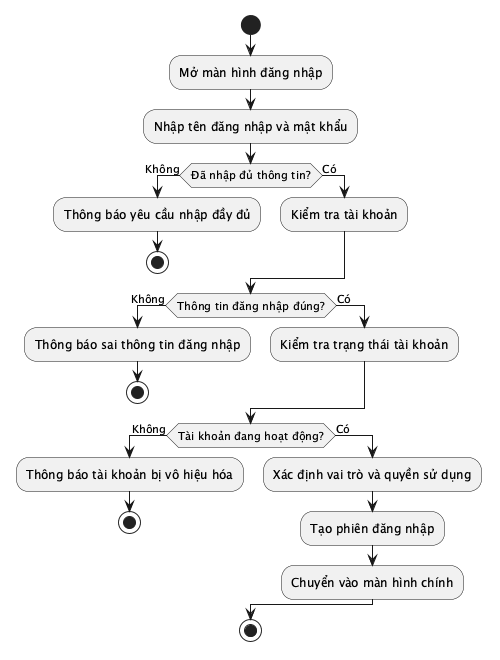
\includegraphics[width=0.95\textwidth,height=0.72\textheight,keepaspectratio]{diagrams/activity-dang-nhap.png}
    \caption{Sơ đồ hoạt động: undefined}
\end{figure}

\textbf{Sơ đồ tuần tự}

\begin{figure}[H]
    \centering
    
\includegraphics[width=0.95\textwidth,height=0.72\textheight,keepaspectratio]{diagrams/sequence-dang-nhap.png}
    \caption{Sơ đồ tuần tự: undefined}
\end{figure}




\subsubsection{Xem tổng quan giảng dạy}

\textbf{Tóm tắt:} Cung cấp số liệu tổng quan về lớp học, học sinh, buổi học và tình hình tài chính.

\textbf{Tác nhân:} Giáo viên

\textbf{Tiền điều kiện}
\begin{itemize}[leftmargin=*]
    \item Giáo viên đã đăng nhập.
\end{itemize}

\textbf{Dòng sự kiện chính}
\begin{enumerate}[leftmargin=*]
    \item Giáo viên truy cập màn hình tổng quan.
    \item Hệ thống tổng hợp dữ liệu lớp học, học sinh, buổi học và tài chính.
    \item Hệ thống hiển thị các chỉ số tổng quan cho giáo viên.
\end{enumerate}

\textbf{Dòng sự kiện phụ}
\begin{itemize}[leftmargin=*]
    \item Nếu không có dữ liệu, hệ thống hiển thị trạng thái trống phù hợp.
\end{itemize}

\textbf{Hậu điều kiện}
\begin{itemize}[leftmargin=*]
    \item Giáo viên nắm được tình hình vận hành hiện tại.
\end{itemize}

\textbf{Sơ đồ luồng dữ liệu}

\begin{figure}[H]
    \centering
    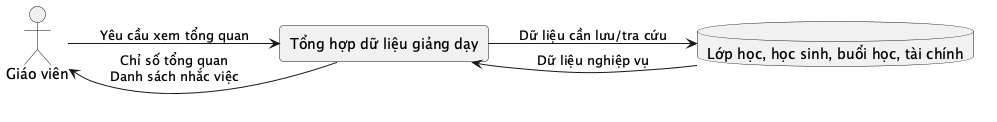
\includegraphics[width=0.95\textwidth,height=0.72\textheight,keepaspectratio]{diagrams/dfd-xem-tong-quan.png}
    \caption{Sơ đồ luồng dữ liệu: undefined}
\end{figure}

\textbf{Sơ đồ hoạt động}

\begin{figure}[H]
    \centering
    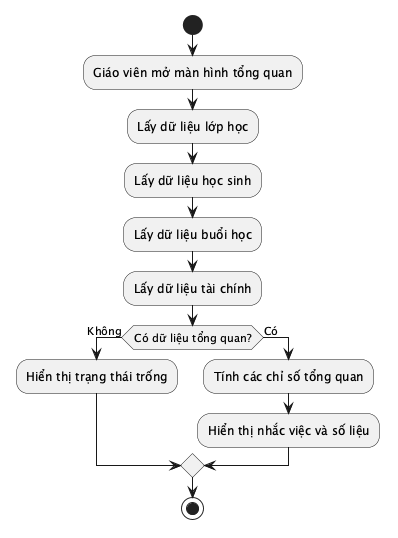
\includegraphics[width=0.95\textwidth,height=0.72\textheight,keepaspectratio]{diagrams/activity-xem-tong-quan.png}
    \caption{Sơ đồ hoạt động: undefined}
\end{figure}






\subsubsection{Cập nhật hồ sơ cá nhân}

\textbf{Tóm tắt:} Cho phép giáo viên cập nhật thông tin hồ sơ cá nhân trong hệ thống.

\textbf{Tác nhân:} Giáo viên

\textbf{Tiền điều kiện}
\begin{itemize}[leftmargin=*]
    \item Giáo viên đã đăng nhập.
\end{itemize}

\textbf{Dòng sự kiện chính}
\begin{enumerate}[leftmargin=*]
    \item Giáo viên mở màn hình hồ sơ cá nhân.
    \item Giáo viên chỉnh sửa thông tin cần thay đổi.
    \item Hệ thống kiểm tra dữ liệu nhập.
    \item Hệ thống lưu thông tin hồ sơ mới.
    \item Hệ thống hiển thị hồ sơ đã cập nhật.
\end{enumerate}

\textbf{Dòng sự kiện phụ}
\begin{itemize}[leftmargin=*]
    \item Nếu dữ liệu không hợp lệ, hệ thống hiển thị lỗi và không lưu thay đổi.
\end{itemize}

\textbf{Hậu điều kiện}
\begin{itemize}[leftmargin=*]
    \item Thông tin hồ sơ cá nhân của giáo viên được cập nhật.
\end{itemize}

\textbf{Sơ đồ luồng dữ liệu}

\begin{figure}[H]
    \centering
    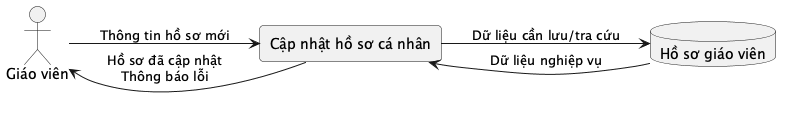
\includegraphics[width=0.95\textwidth,height=0.72\textheight,keepaspectratio]{diagrams/dfd-cap-nhat-ho-so.png}
    \caption{Sơ đồ luồng dữ liệu: undefined}
\end{figure}

\textbf{Sơ đồ hoạt động}

\begin{figure}[H]
    \centering
    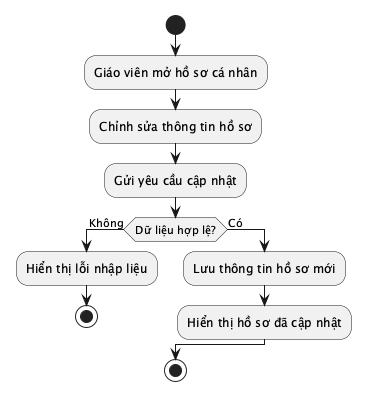
\includegraphics[width=0.95\textwidth,height=0.72\textheight,keepaspectratio]{diagrams/activity-cap-nhat-ho-so.png}
    \caption{Sơ đồ hoạt động: undefined}
\end{figure}






\subsubsection{Liên kết tài khoản Discord}

\textbf{Tóm tắt:} Liên kết tài khoản Discord của giáo viên để hệ thống có thể sử dụng các chức năng Discord liên quan đến lớp học.

\textbf{Tác nhân:} Giáo viên, Discord

\textbf{Tiền điều kiện}
\begin{itemize}[leftmargin=*]
    \item Giáo viên đã đăng nhập.
    \item Bot Discord đã được cấu hình.
\end{itemize}

\textbf{Dòng sự kiện chính}
\begin{enumerate}[leftmargin=*]
    \item Giáo viên chọn liên kết Discord.
    \item Hệ thống chuyển giáo viên sang trang xác thực Discord.
    \item Giáo viên xác nhận quyền truy cập.
    \item Discord trả kết quả xác thực về hệ thống.
    \item Hệ thống lưu định danh Discord của giáo viên.
\end{enumerate}

\textbf{Dòng sự kiện phụ}
\begin{itemize}[leftmargin=*]
    \item Nếu giáo viên hủy xác thực, hệ thống ghi nhận trạng thái hủy.
    \item Nếu Discord trả lỗi hoặc state không hợp lệ, hệ thống thông báo liên kết thất bại.
\end{itemize}

\textbf{Hậu điều kiện}
\begin{itemize}[leftmargin=*]
    \item Tài khoản giáo viên có thông tin Discord đã xác thực.
\end{itemize}

\textbf{Sơ đồ luồng dữ liệu}

\begin{figure}[H]
    \centering
    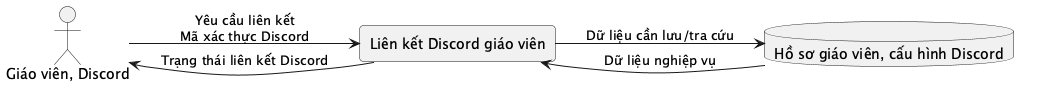
\includegraphics[width=0.95\textwidth,height=0.72\textheight,keepaspectratio]{diagrams/dfd-lien-ket-discord.png}
    \caption{Sơ đồ luồng dữ liệu: undefined}
\end{figure}

\textbf{Sơ đồ hoạt động}

\begin{figure}[H]
    \centering
    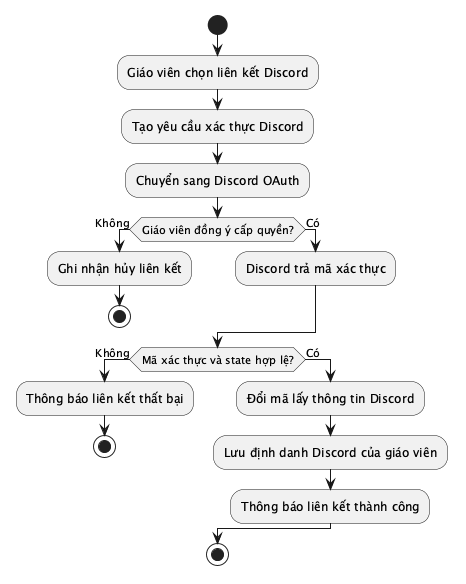
\includegraphics[width=0.95\textwidth,height=0.72\textheight,keepaspectratio]{diagrams/activity-lien-ket-discord.png}
    \caption{Sơ đồ hoạt động: undefined}
\end{figure}






\subsubsection{Quản lý học sinh}

\textbf{Tóm tắt:} Cho phép giáo viên tạo, cập nhật và tra cứu hồ sơ học sinh.

\textbf{Tác nhân:} Giáo viên

\textbf{Tiền điều kiện}
\begin{itemize}[leftmargin=*]
    \item Giáo viên đã đăng nhập.
    \item Lớp học cần ghi danh đang hoạt động.
\end{itemize}

\textbf{Dòng sự kiện chính}
\begin{enumerate}[leftmargin=*]
    \item Giáo viên nhập hoặc chỉnh sửa thông tin học sinh.
    \item Hệ thống kiểm tra tên, lớp học và handle Codeforces.
    \item Hệ thống lưu hồ sơ học sinh.
    \item Khi tạo mới, hệ thống tạo ghi danh học sinh vào lớp.
    \item Hệ thống hiển thị hồ sơ học sinh sau khi lưu.
\end{enumerate}

\textbf{Dòng sự kiện phụ}
\begin{itemize}[leftmargin=*]
    \item Nếu lớp học không tồn tại hoặc đã lưu trữ, hệ thống từ chối thao tác.
    \item Nếu handle Codeforces bị trùng, hệ thống yêu cầu nhập handle khác.
\end{itemize}

\textbf{Hậu điều kiện}
\begin{itemize}[leftmargin=*]
    \item Hồ sơ học sinh được tạo hoặc cập nhật đúng dữ liệu.
\end{itemize}

\textbf{Sơ đồ luồng dữ liệu}

\begin{figure}[H]
    \centering
    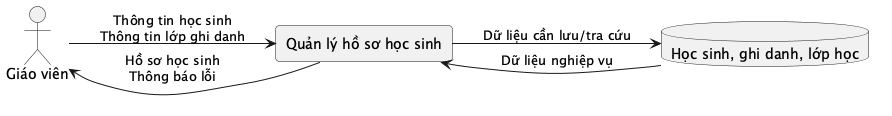
\includegraphics[width=0.95\textwidth,height=0.72\textheight,keepaspectratio]{diagrams/dfd-quan-ly-hoc-sinh.png}
    \caption{Sơ đồ luồng dữ liệu: undefined}
\end{figure}

\textbf{Sơ đồ hoạt động}

\begin{figure}[H]
    \centering
    
\includegraphics[width=0.95\textwidth,height=0.72\textheight,keepaspectratio]{diagrams/activity-quan-ly-hoc-sinh.png}
    \caption{Sơ đồ hoạt động: undefined}
\end{figure}






\subsubsection{Quản lý ghi danh học sinh}

\textbf{Tóm tắt:} Quản lý việc chuyển lớp, nghỉ học, lưu trữ và học lại của học sinh.

\textbf{Tác nhân:} Giáo viên

\textbf{Tiền điều kiện}
\begin{itemize}[leftmargin=*]
    \item Giáo viên đã đăng nhập.
    \item Học sinh đã tồn tại trong hệ thống.
\end{itemize}

\textbf{Dòng sự kiện chính}
\begin{enumerate}[leftmargin=*]
    \item Giáo viên chọn học sinh và thao tác ghi danh cần thực hiện.
    \item Hệ thống kiểm tra trạng thái hiện tại của học sinh.
    \item Hệ thống kiểm tra lớp đích hoặc thời điểm thay đổi.
    \item Hệ thống kết thúc ghi danh cũ nếu cần.
    \item Hệ thống tạo ghi danh mới hoặc cập nhật trạng thái học sinh.
    \item Hệ thống hiển thị trạng thái học sinh sau thao tác.
\end{enumerate}

\textbf{Dòng sự kiện phụ}
\begin{itemize}[leftmargin=*]
    \item Nếu chuyển về chính lớp hiện tại, hệ thống từ chối thao tác.
    \item Nếu thời điểm thay đổi không hợp lệ, hệ thống thông báo lỗi.
    \item Nếu học sinh còn công nợ khi nghỉ học, hệ thống chuyển sang trạng thái chờ lưu trữ.
\end{itemize}

\textbf{Hậu điều kiện}
\begin{itemize}[leftmargin=*]
    \item Trạng thái học sinh và lịch sử ghi danh được cập nhật nhất quán.
\end{itemize}

\textbf{Sơ đồ luồng dữ liệu}

\begin{figure}[H]
    \centering
    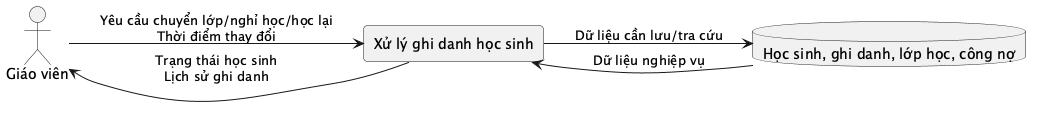
\includegraphics[width=0.95\textwidth,height=0.72\textheight,keepaspectratio]{diagrams/dfd-quan-ly-ghi-danh.png}
    \caption{Sơ đồ luồng dữ liệu: undefined}
\end{figure}

\textbf{Sơ đồ hoạt động}

\begin{figure}[H]
    \centering
    
\includegraphics[width=0.95\textwidth,height=0.72\textheight,keepaspectratio]{diagrams/activity-quan-ly-ghi-danh.png}
    \caption{Sơ đồ hoạt động: undefined}
\end{figure}

\textbf{Sơ đồ tuần tự}

\begin{figure}[H]
    \centering
    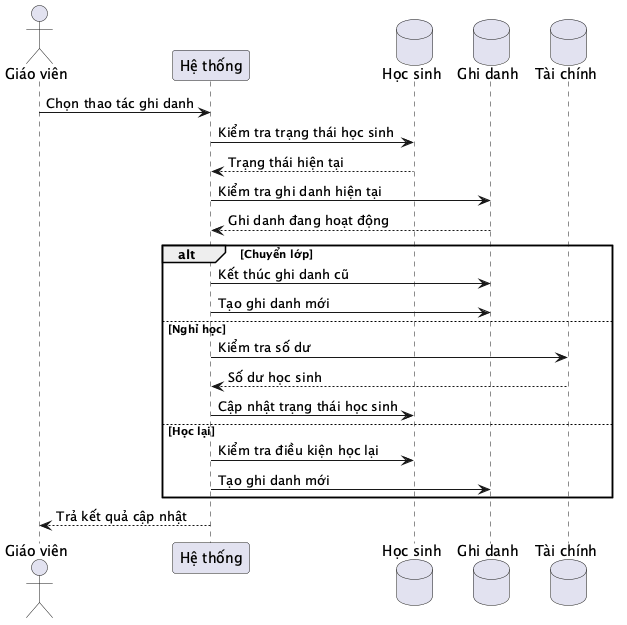
\includegraphics[width=0.95\textwidth,height=0.72\textheight,keepaspectratio]{diagrams/sequence-ghi-danh.png}
    \caption{Sơ đồ tuần tự: undefined}
\end{figure}

\textbf{Sơ đồ cộng tác}

\begin{figure}[H]
    \centering
    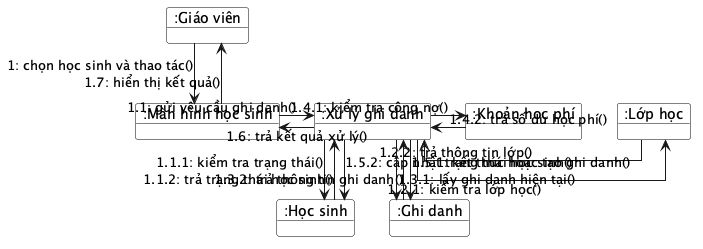
\includegraphics[width=0.95\textwidth,height=0.72\textheight,keepaspectratio]{diagrams/collaboration-ghi-danh.png}
    \caption{Sơ đồ cộng tác: undefined}
\end{figure}


\subsubsection{Xử lý học sinh chờ lưu trữ}

\textbf{Tóm tắt:} Hoàn tất lưu trữ học sinh sau khi các khoản phải thu hoặc hoàn trả đã được xử lý.

\textbf{Tác nhân:} Giáo viên

\textbf{Tiền điều kiện}
\begin{itemize}[leftmargin=*]
    \item Học sinh đang ở trạng thái chờ lưu trữ.
\end{itemize}

\textbf{Dòng sự kiện chính}
\begin{enumerate}[leftmargin=*]
    \item Giáo viên mở danh sách học sinh chờ lưu trữ.
    \item Giáo viên chọn học sinh cần lưu trữ.
    \item Hệ thống kiểm tra số dư công nợ của học sinh.
    \item Nếu số dư bằng 0, hệ thống lưu trữ học sinh.
    \item Hệ thống cập nhật danh sách chờ lưu trữ.
\end{enumerate}

\textbf{Dòng sự kiện phụ}
\begin{itemize}[leftmargin=*]
    \item Nếu số dư khác 0, hệ thống yêu cầu xử lý tài chính trước khi lưu trữ.
\end{itemize}

\textbf{Hậu điều kiện}
\begin{itemize}[leftmargin=*]
    \item Học sinh được lưu trữ khi đủ điều kiện.
\end{itemize}

\textbf{Sơ đồ luồng dữ liệu}

\begin{figure}[H]
    \centering
    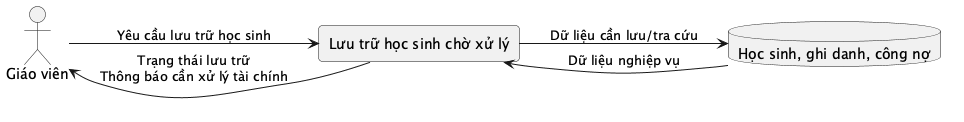
\includegraphics[width=0.95\textwidth,height=0.72\textheight,keepaspectratio]{diagrams/dfd-xu-ly-cho-luu-tru.png}
    \caption{Sơ đồ luồng dữ liệu: undefined}
\end{figure}

\textbf{Sơ đồ hoạt động}

\begin{figure}[H]
    \centering
    
\includegraphics[width=0.95\textwidth,height=0.72\textheight,keepaspectratio]{diagrams/activity-xu-ly-cho-luu-tru.png}
    \caption{Sơ đồ hoạt động: undefined}
\end{figure}






\subsubsection{Quản lý lớp học}

\textbf{Tóm tắt:} Cho phép giáo viên tạo, cập nhật và lưu trữ lớp học.

\textbf{Tác nhân:} Giáo viên

\textbf{Tiền điều kiện}
\begin{itemize}[leftmargin=*]
    \item Giáo viên đã đăng nhập.
\end{itemize}

\textbf{Dòng sự kiện chính}
\begin{enumerate}[leftmargin=*]
    \item Giáo viên nhập thông tin lớp học.
    \item Hệ thống kiểm tra tên lớp, học phí và lịch học.
    \item Hệ thống lưu thông tin lớp học.
    \item Hệ thống lưu lịch học định kỳ kèm theo nếu có.
    \item Hệ thống hiển thị lớp học đã cập nhật.
\end{enumerate}

\textbf{Dòng sự kiện phụ}
\begin{itemize}[leftmargin=*]
    \item Nếu tên lớp, học phí hoặc lịch học không hợp lệ, hệ thống thông báo lỗi.
\end{itemize}

\textbf{Hậu điều kiện}
\begin{itemize}[leftmargin=*]
    \item Thông tin lớp học được lưu đúng trạng thái.
\end{itemize}

\textbf{Sơ đồ luồng dữ liệu}

\begin{figure}[H]
    \centering
    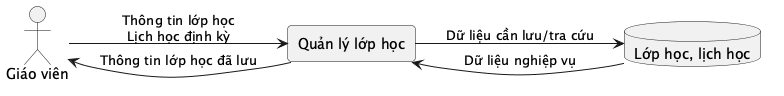
\includegraphics[width=0.95\textwidth,height=0.72\textheight,keepaspectratio]{diagrams/dfd-quan-ly-lop-hoc.png}
    \caption{Sơ đồ luồng dữ liệu: undefined}
\end{figure}

\textbf{Sơ đồ hoạt động}

\begin{figure}[H]
    \centering
    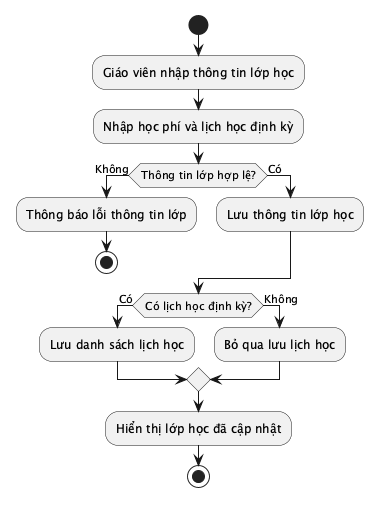
\includegraphics[width=0.95\textwidth,height=0.72\textheight,keepaspectratio]{diagrams/activity-quan-ly-lop-hoc.png}
    \caption{Sơ đồ hoạt động: undefined}
\end{figure}






\subsubsection{Quản lý lịch học định kỳ}

\textbf{Tóm tắt:} Quản lý các khung giờ học định kỳ của một lớp.

\textbf{Tác nhân:} Giáo viên

\textbf{Tiền điều kiện}
\begin{itemize}[leftmargin=*]
    \item Lớp học tồn tại và đang hoạt động.
\end{itemize}

\textbf{Dòng sự kiện chính}
\begin{enumerate}[leftmargin=*]
    \item Giáo viên mở thông tin lịch học của lớp.
    \item Giáo viên thêm, sửa hoặc thay thế lịch định kỳ.
    \item Hệ thống lưu lịch học mới.
    \item Hệ thống hiển thị danh sách lịch học đã cập nhật.
\end{enumerate}

\textbf{Dòng sự kiện phụ}
\begin{itemize}[leftmargin=*]
    \item Nếu lịch học không hợp lệ, hệ thống yêu cầu chỉnh sửa lại.
\end{itemize}

\textbf{Hậu điều kiện}
\begin{itemize}[leftmargin=*]
    \item Lịch học định kỳ của lớp được cập nhật.
\end{itemize}

\textbf{Sơ đồ luồng dữ liệu}

\begin{figure}[H]
    \centering
    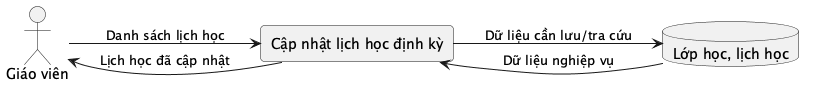
\includegraphics[width=0.95\textwidth,height=0.72\textheight,keepaspectratio]{diagrams/dfd-quan-ly-lich-hoc.png}
    \caption{Sơ đồ luồng dữ liệu: undefined}
\end{figure}

\textbf{Sơ đồ hoạt động}

\begin{figure}[H]
    \centering
    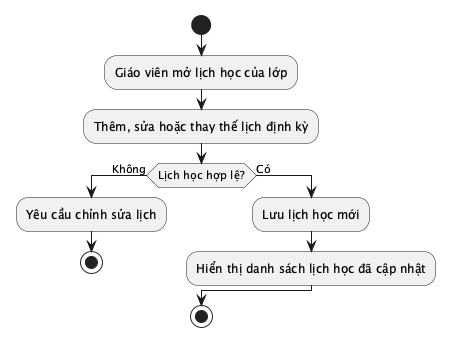
\includegraphics[width=0.95\textwidth,height=0.72\textheight,keepaspectratio]{diagrams/activity-quan-ly-lich-hoc.png}
    \caption{Sơ đồ hoạt động: undefined}
\end{figure}






\subsubsection{Quản lý buổi học}

\textbf{Tóm tắt:} Cho phép giáo viên xem, tạo thủ công và hủy buổi học.

\textbf{Tác nhân:} Giáo viên

\textbf{Tiền điều kiện}
\begin{itemize}[leftmargin=*]
    \item Giáo viên đã đăng nhập.
    \item Lớp học đang hoạt động.
\end{itemize}

\textbf{Dòng sự kiện chính}
\begin{enumerate}[leftmargin=*]
    \item Giáo viên mở danh sách buổi học.
    \item Giáo viên tạo buổi học thủ công hoặc chọn hủy buổi học.
    \item Hệ thống kiểm tra lớp, thời gian, trùng lịch và giao nhau.
    \item Hệ thống lưu buổi học hoặc cập nhật trạng thái hủy.
    \item Hệ thống hiển thị danh sách buổi học mới.
\end{enumerate}

\textbf{Dòng sự kiện phụ}
\begin{itemize}[leftmargin=*]
    \item Nếu thời gian nằm trong quá khứ, hệ thống từ chối tạo buổi học.
    \item Nếu buổi học bị trùng hoặc giao nhau, hệ thống thông báo lỗi.
\end{itemize}

\textbf{Hậu điều kiện}
\begin{itemize}[leftmargin=*]
    \item Buổi học được tạo hoặc hủy theo đúng quy tắc.
\end{itemize}

\textbf{Sơ đồ luồng dữ liệu}

\begin{figure}[H]
    \centering
    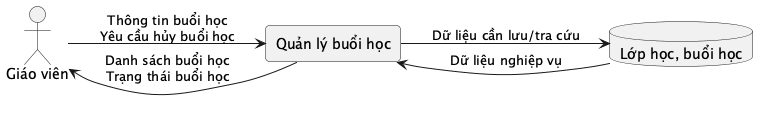
\includegraphics[width=0.95\textwidth,height=0.72\textheight,keepaspectratio]{diagrams/dfd-quan-ly-buoi-hoc.png}
    \caption{Sơ đồ luồng dữ liệu: undefined}
\end{figure}

\textbf{Sơ đồ hoạt động}

\begin{figure}[H]
    \centering
    
\includegraphics[width=0.95\textwidth,height=0.72\textheight,keepaspectratio]{diagrams/activity-quan-ly-buoi-hoc.png}
    \caption{Sơ đồ hoạt động: undefined}
\end{figure}






\subsubsection{Điểm danh buổi học}

\textbf{Tóm tắt:} Ghi nhận tình trạng tham gia buổi học của học sinh và đồng bộ khoản học phí phát sinh.

\textbf{Tác nhân:} Giáo viên, Discord

\textbf{Tiền điều kiện}
\begin{itemize}[leftmargin=*]
    \item Buổi học tồn tại và chưa bị hủy.
    \item Học sinh có ghi danh hợp lệ tại thời điểm buổi học.
\end{itemize}

\textbf{Dòng sự kiện chính}
\begin{enumerate}[leftmargin=*]
    \item Giáo viên mở chi tiết điểm danh của buổi học.
    \item Hệ thống hiển thị danh sách học sinh thuộc lớp tại thời điểm buổi học.
    \item Giáo viên cập nhật trạng thái điểm danh.
    \item Hệ thống kiểm tra học sinh còn ghi danh hợp lệ.
    \item Hệ thống lưu bản ghi điểm danh.
    \item Hệ thống tạo, kích hoạt hoặc hủy khoản học phí tương ứng.
\end{enumerate}

\textbf{Dòng sự kiện phụ}
\begin{itemize}[leftmargin=*]
    \item Nếu buổi học đã hủy, hệ thống không cho cập nhật điểm danh.
    \item Nếu học sinh không thuộc lớp tại thời điểm buổi học, hệ thống từ chối cập nhật.
    \item Nếu có dữ liệu voice từ Discord, hệ thống có thể tự ghi nhận điểm danh trước khi giáo viên ghi đè thủ công.
\end{itemize}

\textbf{Hậu điều kiện}
\begin{itemize}[leftmargin=*]
    \item Điểm danh và khoản học phí phát sinh được cập nhật nhất quán.
\end{itemize}

\textbf{Sơ đồ luồng dữ liệu}

\begin{figure}[H]
    \centering
    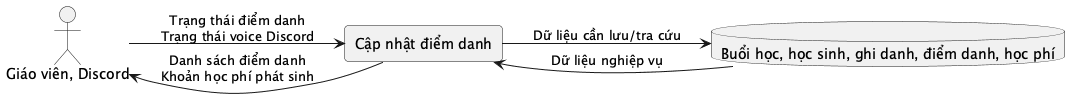
\includegraphics[width=0.95\textwidth,height=0.72\textheight,keepaspectratio]{diagrams/dfd-diem-danh-buoi-hoc.png}
    \caption{Sơ đồ luồng dữ liệu: undefined}
\end{figure}

\textbf{Sơ đồ hoạt động}

\begin{figure}[H]
    \centering
    
\includegraphics[width=0.95\textwidth,height=0.72\textheight,keepaspectratio]{diagrams/activity-diem-danh-buoi-hoc.png}
    \caption{Sơ đồ hoạt động: undefined}
\end{figure}

\textbf{Sơ đồ tuần tự}

\begin{figure}[H]
    \centering
    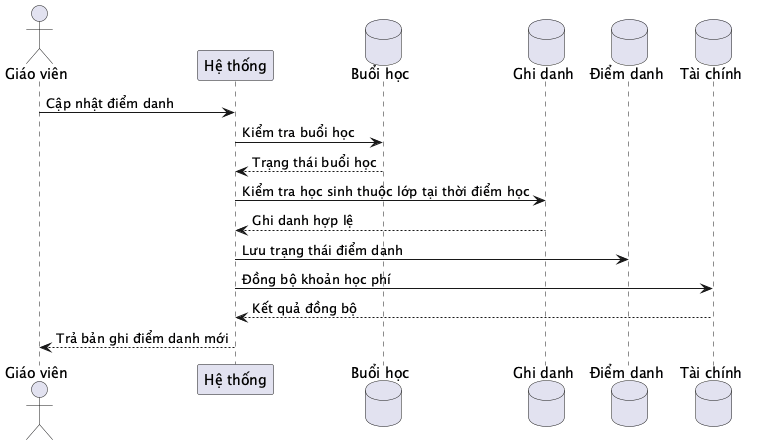
\includegraphics[width=0.95\textwidth,height=0.72\textheight,keepaspectratio]{diagrams/sequence-diem-danh.png}
    \caption{Sơ đồ tuần tự: undefined}
\end{figure}

\textbf{Sơ đồ cộng tác}

\begin{figure}[H]
    \centering
    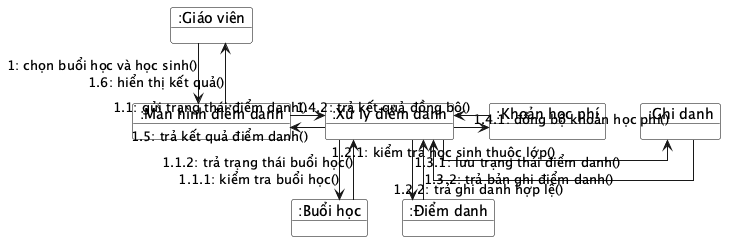
\includegraphics[width=0.95\textwidth,height=0.72\textheight,keepaspectratio]{diagrams/collaboration-diem-danh.png}
    \caption{Sơ đồ cộng tác: undefined}
\end{figure}


\subsubsection{Theo dõi kết quả học tập}

\textbf{Tóm tắt:} Cho phép giáo viên xem hồ sơ học tập và tiến độ của học sinh.

\textbf{Tác nhân:} Giáo viên

\textbf{Tiền điều kiện}
\begin{itemize}[leftmargin=*]
    \item Giáo viên đã đăng nhập.
    \item Học sinh tồn tại trong hệ thống.
\end{itemize}

\textbf{Dòng sự kiện chính}
\begin{enumerate}[leftmargin=*]
    \item Giáo viên mở hồ sơ học tập của học sinh.
    \item Hệ thống tổng hợp ghi danh, điểm danh, tài chính và kết quả liên quan.
    \item Hệ thống hiển thị hồ sơ học tập cho giáo viên.
\end{enumerate}

\textbf{Dòng sự kiện phụ}
\begin{itemize}[leftmargin=*]
    \item Nếu học sinh không tồn tại, hệ thống thông báo không tìm thấy dữ liệu.
\end{itemize}

\textbf{Hậu điều kiện}
\begin{itemize}[leftmargin=*]
    \item Giáo viên xem được thông tin học tập tổng hợp của học sinh.
\end{itemize}

\textbf{Sơ đồ luồng dữ liệu}

\begin{figure}[H]
    \centering
    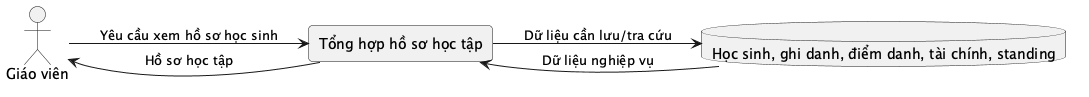
\includegraphics[width=0.95\textwidth,height=0.72\textheight,keepaspectratio]{diagrams/dfd-theo-doi-ket-qua.png}
    \caption{Sơ đồ luồng dữ liệu: undefined}
\end{figure}

\textbf{Sơ đồ hoạt động}

\begin{figure}[H]
    \centering
    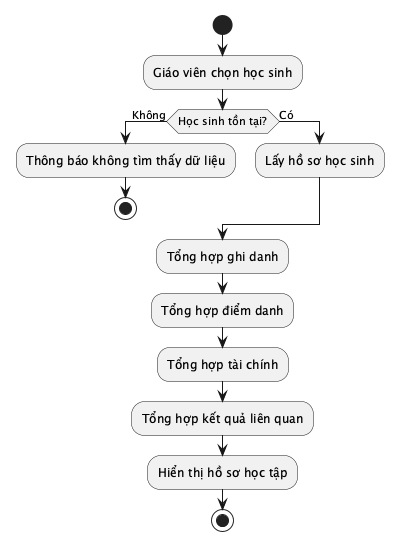
\includegraphics[width=0.95\textwidth,height=0.72\textheight,keepaspectratio]{diagrams/activity-theo-doi-ket-qua.png}
    \caption{Sơ đồ hoạt động: undefined}
\end{figure}






\subsubsection{Quản lý giao dịch tài chính}

\textbf{Tóm tắt:} Ghi nhận các giao dịch thu tiền, hoàn trả và cập nhật trạng thái khoản học phí.

\textbf{Tác nhân:} Giáo viên

\textbf{Tiền điều kiện}
\begin{itemize}[leftmargin=*]
    \item Giáo viên đã đăng nhập.
    \item Học sinh liên quan tồn tại trong hệ thống.
\end{itemize}

\textbf{Dòng sự kiện chính}
\begin{enumerate}[leftmargin=*]
    \item Giáo viên nhập giao dịch tài chính.
    \item Hệ thống kiểm tra học sinh, số tiền, loại giao dịch và ngày ghi nhận.
    \item Hệ thống lưu giao dịch.
    \item Giáo viên có thể cập nhật trạng thái khoản học phí phát sinh.
    \item Hệ thống hiển thị danh sách giao dịch mới.
\end{enumerate}

\textbf{Dòng sự kiện phụ}
\begin{itemize}[leftmargin=*]
    \item Nếu số tiền hoặc học sinh không hợp lệ, hệ thống thông báo lỗi.
\end{itemize}

\textbf{Hậu điều kiện}
\begin{itemize}[leftmargin=*]
    \item Dữ liệu giao dịch và trạng thái khoản học phí được cập nhật.
\end{itemize}

\textbf{Sơ đồ luồng dữ liệu}

\begin{figure}[H]
    \centering
    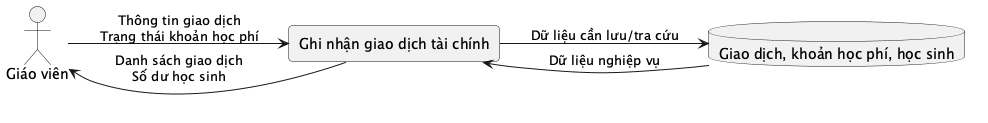
\includegraphics[width=0.95\textwidth,height=0.72\textheight,keepaspectratio]{diagrams/dfd-quan-ly-giao-dich.png}
    \caption{Sơ đồ luồng dữ liệu: undefined}
\end{figure}

\textbf{Sơ đồ hoạt động}

\begin{figure}[H]
    \centering
    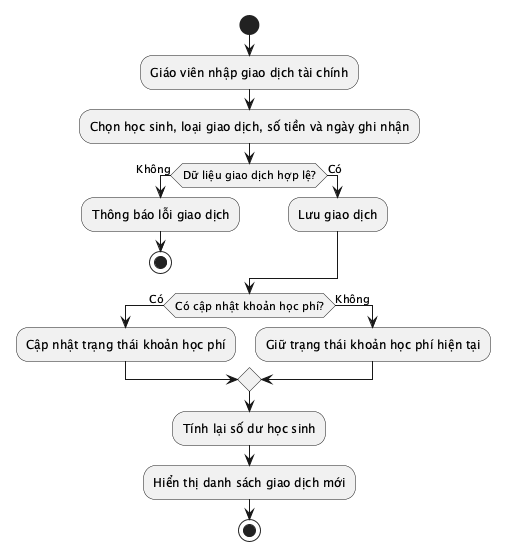
\includegraphics[width=0.95\textwidth,height=0.72\textheight,keepaspectratio]{diagrams/activity-quan-ly-giao-dich.png}
    \caption{Sơ đồ hoạt động: undefined}
\end{figure}






\subsubsection{Xem báo cáo tài chính}

\textbf{Tóm tắt:} Cung cấp báo cáo thu chi, công nợ và số dư học sinh.

\textbf{Tác nhân:} Giáo viên

\textbf{Tiền điều kiện}
\begin{itemize}[leftmargin=*]
    \item Giáo viên đã đăng nhập.
\end{itemize}

\textbf{Dòng sự kiện chính}
\begin{enumerate}[leftmargin=*]
    \item Giáo viên mở màn hình báo cáo tài chính.
    \item Giáo viên chọn bộ lọc thời gian hoặc lớp học.
    \item Hệ thống tổng hợp giao dịch, khoản học phí và số dư.
    \item Hệ thống hiển thị báo cáo tài chính.
\end{enumerate}

\textbf{Dòng sự kiện phụ}
\begin{itemize}[leftmargin=*]
    \item Nếu không có dữ liệu, hệ thống hiển thị báo cáo rỗng.
\end{itemize}

\textbf{Hậu điều kiện}
\begin{itemize}[leftmargin=*]
    \item Giáo viên xem được tình hình tài chính theo bộ lọc.
\end{itemize}

\textbf{Sơ đồ luồng dữ liệu}

\begin{figure}[H]
    \centering
    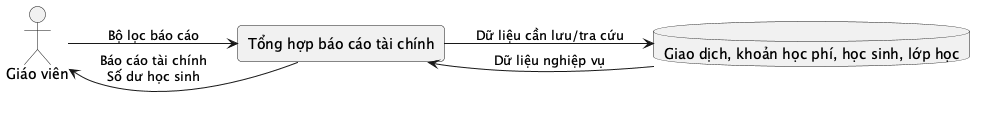
\includegraphics[width=0.95\textwidth,height=0.72\textheight,keepaspectratio]{diagrams/dfd-xem-bao-cao-tai-chinh.png}
    \caption{Sơ đồ luồng dữ liệu: undefined}
\end{figure}

\textbf{Sơ đồ hoạt động}

\begin{figure}[H]
    \centering
    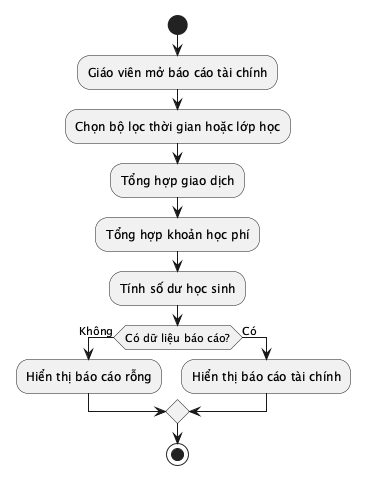
\includegraphics[width=0.95\textwidth,height=0.72\textheight,keepaspectratio]{diagrams/activity-xem-bao-cao-tai-chinh.png}
    \caption{Sơ đồ hoạt động: undefined}
\end{figure}






\subsubsection{Thiết lập Discord cho lớp học}

\textbf{Tóm tắt:} Gắn Discord Guild và các kênh cần thiết với một lớp học.

\textbf{Tác nhân:} Giáo viên, Discord

\textbf{Tiền điều kiện}
\begin{itemize}[leftmargin=*]
    \item Giáo viên đã liên kết Discord.
    \item Bot Discord đã được cài vào guild cần sử dụng.
\end{itemize}

\textbf{Dòng sự kiện chính}
\begin{enumerate}[leftmargin=*]
    \item Giáo viên mở phần thiết lập Discord của lớp.
    \item Hệ thống lấy danh sách guild và channel từ dữ liệu Discord đã đồng bộ.
    \item Giáo viên chọn guild, kênh thông báo và kênh voice điểm danh.
    \item Hệ thống kiểm tra guild chưa bị gắn cho lớp khác.
    \item Hệ thống kiểm tra đúng loại kênh text/voice.
    \item Hệ thống lưu thiết lập Discord cho lớp.
\end{enumerate}

\textbf{Dòng sự kiện phụ}
\begin{itemize}[leftmargin=*]
    \item Nếu guild đã được gắn với lớp khác, hệ thống từ chối.
    \item Nếu chọn sai loại kênh, hệ thống yêu cầu chọn lại.
\end{itemize}

\textbf{Hậu điều kiện}
\begin{itemize}[leftmargin=*]
    \item Lớp học có cấu hình Discord hợp lệ.
\end{itemize}

\textbf{Sơ đồ luồng dữ liệu}

\begin{figure}[H]
    \centering
    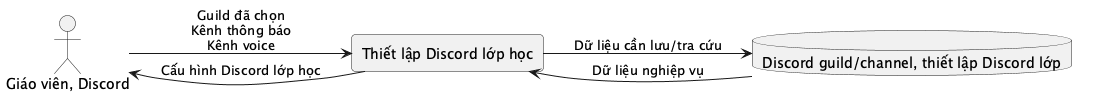
\includegraphics[width=0.95\textwidth,height=0.72\textheight,keepaspectratio]{diagrams/dfd-thiet-lap-discord-lop.png}
    \caption{Sơ đồ luồng dữ liệu: undefined}
\end{figure}

\textbf{Sơ đồ hoạt động}

\begin{figure}[H]
    \centering
    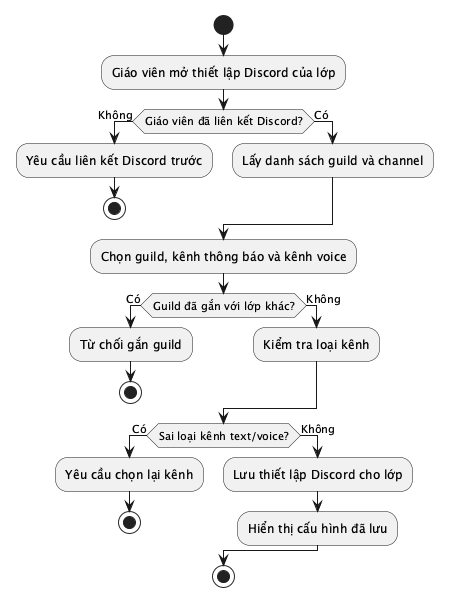
\includegraphics[width=0.95\textwidth,height=0.72\textheight,keepaspectratio]{diagrams/activity-thiet-lap-discord-lop.png}
    \caption{Sơ đồ hoạt động: undefined}
\end{figure}






\subsubsection{Gửi thông báo cho học sinh}

\textbf{Tóm tắt:} Gửi thông báo đến học sinh hoặc lớp thông qua Discord.

\textbf{Tác nhân:} Giáo viên, Discord

\textbf{Tiền điều kiện}
\begin{itemize}[leftmargin=*]
    \item Giáo viên đã đăng nhập.
    \item Lớp hoặc học sinh nhận thông báo có cấu hình Discord phù hợp.
\end{itemize}

\textbf{Dòng sự kiện chính}
\begin{enumerate}[leftmargin=*]
    \item Giáo viên nhập nội dung thông báo và chọn người nhận.
    \item Hệ thống xác định danh sách người nhận hoặc kênh nhận.
    \item Hệ thống kiểm tra cấu hình Discord liên quan.
    \item Hệ thống gửi thông báo qua Discord.
    \item Hệ thống trả kết quả gửi thành công/thất bại cho từng đích.
\end{enumerate}

\textbf{Dòng sự kiện phụ}
\begin{itemize}[leftmargin=*]
    \item Nếu học sinh chưa có Discord hoặc lớp chưa cấu hình guild, hệ thống ghi nhận gửi thất bại cho đích đó.
    \item Nếu Discord trả lỗi, hệ thống hiển thị chi tiết lỗi tương ứng.
\end{itemize}

\textbf{Hậu điều kiện}
\begin{itemize}[leftmargin=*]
    \item Thông báo được gửi đến các đích hợp lệ và kết quả gửi được hiển thị.
\end{itemize}

\textbf{Sơ đồ luồng dữ liệu}

\begin{figure}[H]
    \centering
    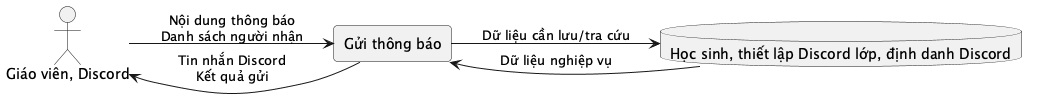
\includegraphics[width=0.95\textwidth,height=0.72\textheight,keepaspectratio]{diagrams/dfd-gui-thong-bao.png}
    \caption{Sơ đồ luồng dữ liệu: undefined}
\end{figure}

\textbf{Sơ đồ hoạt động}

\begin{figure}[H]
    \centering
    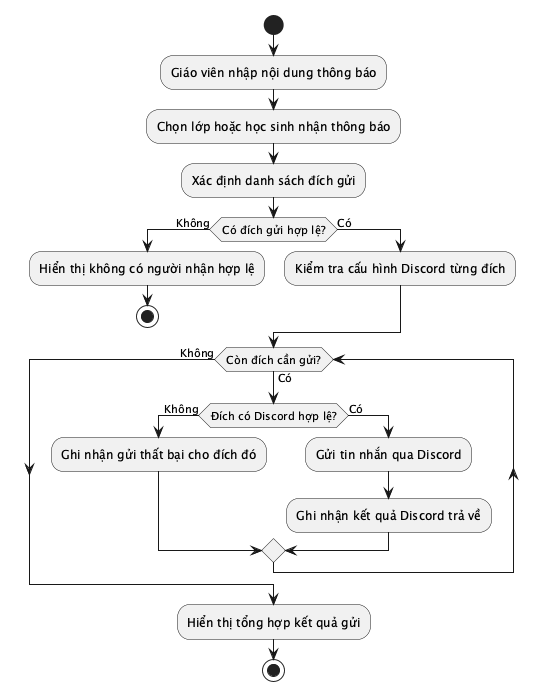
\includegraphics[width=0.95\textwidth,height=0.72\textheight,keepaspectratio]{diagrams/activity-gui-thong-bao.png}
    \caption{Sơ đồ hoạt động: undefined}
\end{figure}






\subsubsection{Gắn Gym Codeforces cho lớp học}

\textbf{Tóm tắt:} Gắn một Gym Codeforces đã đồng bộ vào lớp học để theo dõi bài tập và standing.

\textbf{Tác nhân:} Giáo viên, Codeforces

\textbf{Tiền điều kiện}
\begin{itemize}[leftmargin=*]
    \item Lớp học đang hoạt động.
    \item Gym đã được đồng bộ từ Codeforces.
\end{itemize}

\textbf{Dòng sự kiện chính}
\begin{enumerate}[leftmargin=*]
    \item Giáo viên mở danh sách Gym có thể gắn.
    \item Giáo viên chọn Gym cần gắn cho lớp.
    \item Hệ thống kiểm tra lớp học và Gym đã đồng bộ.
    \item Hệ thống tạo Gym gắn với lớp.
    \item Hệ thống hiển thị Gym trong lớp học.
\end{enumerate}

\textbf{Dòng sự kiện phụ}
\begin{itemize}[leftmargin=*]
    \item Nếu lớp đã lưu trữ, hệ thống từ chối thao tác.
    \item Nếu Gym chưa được đồng bộ, hệ thống thông báo không tìm thấy Gym.
\end{itemize}

\textbf{Hậu điều kiện}
\begin{itemize}[leftmargin=*]
    \item Lớp học có Gym Codeforces để theo dõi standing.
\end{itemize}

\textbf{Sơ đồ luồng dữ liệu}

\begin{figure}[H]
    \centering
    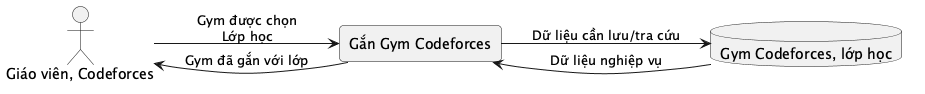
\includegraphics[width=0.95\textwidth,height=0.72\textheight,keepaspectratio]{diagrams/dfd-gan-gym-codeforces.png}
    \caption{Sơ đồ luồng dữ liệu: undefined}
\end{figure}

\textbf{Sơ đồ hoạt động}

\begin{figure}[H]
    \centering
    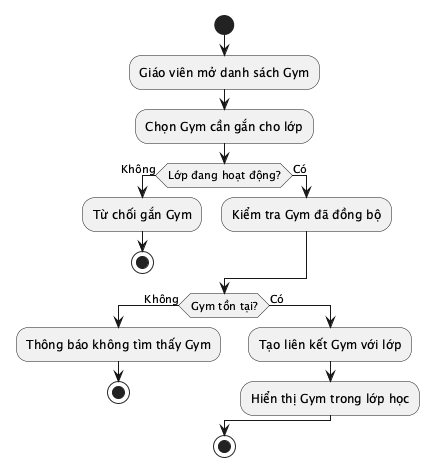
\includegraphics[width=0.95\textwidth,height=0.72\textheight,keepaspectratio]{diagrams/activity-gan-gym-codeforces.png}
    \caption{Sơ đồ hoạt động: undefined}
\end{figure}






\subsubsection{Xem bảng xếp hạng Gym}

\textbf{Tóm tắt:} Hiển thị standing của học sinh trong một Gym Codeforces đã gắn với lớp.

\textbf{Tác nhân:} Giáo viên, Codeforces

\textbf{Tiền điều kiện}
\begin{itemize}[leftmargin=*]
    \item Lớp học đã gắn Gym Codeforces.
    \item Dữ liệu standing đã được đồng bộ.
\end{itemize}

\textbf{Dòng sự kiện chính}
\begin{enumerate}[leftmargin=*]
    \item Giáo viên mở bảng xếp hạng Gym của lớp.
    \item Hệ thống đọc dữ liệu bài tập và standing đã đồng bộ.
    \item Hệ thống ghép standing với danh sách học sinh của lớp.
    \item Hệ thống hiển thị ma trận kết quả.
\end{enumerate}

\textbf{Dòng sự kiện phụ}
\begin{itemize}[leftmargin=*]
    \item Nếu chưa có dữ liệu standing, hệ thống hiển thị trạng thái chưa có dữ liệu.
\end{itemize}

\textbf{Hậu điều kiện}
\begin{itemize}[leftmargin=*]
    \item Giáo viên xem được kết quả làm bài của học sinh trong Gym.
\end{itemize}

\textbf{Sơ đồ luồng dữ liệu}

\begin{figure}[H]
    \centering
    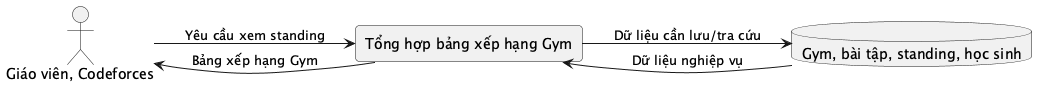
\includegraphics[width=0.95\textwidth,height=0.72\textheight,keepaspectratio]{diagrams/dfd-xem-bang-xep-hang.png}
    \caption{Sơ đồ luồng dữ liệu: undefined}
\end{figure}

\textbf{Sơ đồ hoạt động}

\begin{figure}[H]
    \centering
    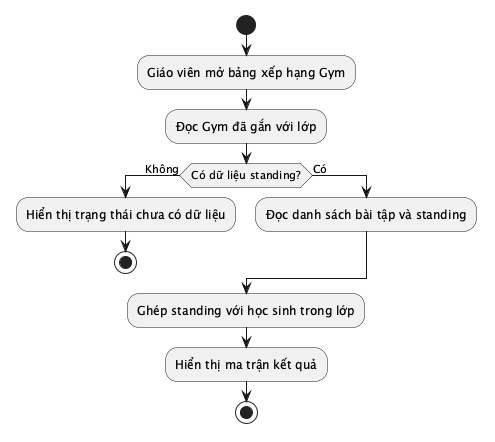
\includegraphics[width=0.95\textwidth,height=0.72\textheight,keepaspectratio]{diagrams/activity-xem-bang-xep-hang.png}
    \caption{Sơ đồ hoạt động: undefined}
\end{figure}






\subsubsection{Quản lý tài khoản giáo viên}

\textbf{Tóm tắt:} Cho phép quản trị viên xem và cập nhật tài khoản giáo viên.

\textbf{Tác nhân:} Quản trị viên

\textbf{Tiền điều kiện}
\begin{itemize}[leftmargin=*]
    \item Quản trị viên đã đăng nhập.
\end{itemize}

\textbf{Dòng sự kiện chính}
\begin{enumerate}[leftmargin=*]
    \item Quản trị viên mở danh sách tài khoản giáo viên.
    \item Hệ thống hiển thị danh sách tài khoản.
    \item Quản trị viên cập nhật thông tin hoặc trạng thái tài khoản.
    \item Hệ thống lưu thay đổi.
    \item Hệ thống hiển thị tài khoản đã cập nhật.
\end{enumerate}

\textbf{Dòng sự kiện phụ}
\begin{itemize}[leftmargin=*]
    \item Nếu tài khoản không tồn tại, hệ thống thông báo lỗi.
\end{itemize}

\textbf{Hậu điều kiện}
\begin{itemize}[leftmargin=*]
    \item Tài khoản giáo viên được cập nhật theo thao tác quản trị.
\end{itemize}

\textbf{Sơ đồ luồng dữ liệu}

\begin{figure}[H]
    \centering
    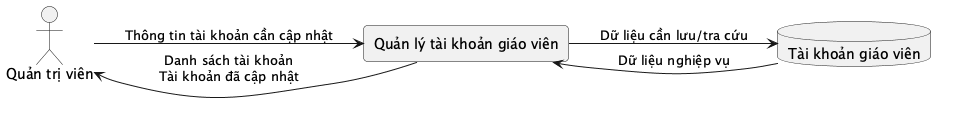
\includegraphics[width=0.95\textwidth,height=0.72\textheight,keepaspectratio]{diagrams/dfd-quan-ly-tai-khoan-giao-vien.png}
    \caption{Sơ đồ luồng dữ liệu: undefined}
\end{figure}

\textbf{Sơ đồ hoạt động}

\begin{figure}[H]
    \centering
    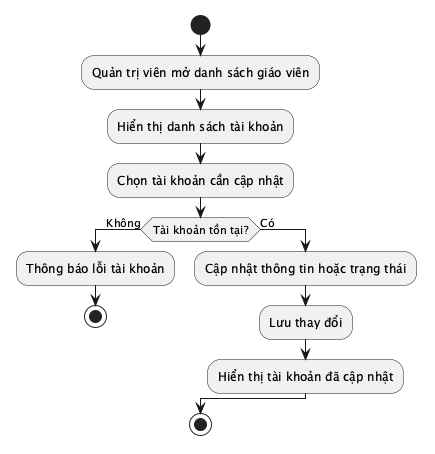
\includegraphics[width=0.95\textwidth,height=0.72\textheight,keepaspectratio]{diagrams/activity-quan-ly-tai-khoan-giao-vien.png}
    \caption{Sơ đồ hoạt động: undefined}
\end{figure}






\subsubsection{Cấu hình bot Discord}

\textbf{Tóm tắt:} Lưu cấu hình bot Discord để hệ thống sử dụng cho các chức năng Discord.

\textbf{Tác nhân:} Quản trị viên

\textbf{Tiền điều kiện}
\begin{itemize}[leftmargin=*]
    \item Quản trị viên đã đăng nhập.
    \item Thông tin bot Discord hợp lệ đã được chuẩn bị.
\end{itemize}

\textbf{Dòng sự kiện chính}
\begin{enumerate}[leftmargin=*]
    \item Quản trị viên mở màn hình cấu hình Discord.
    \item Quản trị viên nhập bot token, client id, client secret và quyền cần dùng.
    \item Hệ thống kiểm tra dữ liệu cấu hình.
    \item Hệ thống lưu cấu hình bot Discord.
    \item Hệ thống hiển thị trạng thái cấu hình.
\end{enumerate}

\textbf{Dòng sự kiện phụ}
\begin{itemize}[leftmargin=*]
    \item Nếu thiếu thông tin bắt buộc, hệ thống yêu cầu nhập đầy đủ.
\end{itemize}

\textbf{Hậu điều kiện}
\begin{itemize}[leftmargin=*]
    \item Bot Discord được cấu hình để phục vụ các luồng Discord của hệ thống.
\end{itemize}

\textbf{Sơ đồ luồng dữ liệu}

\begin{figure}[H]
    \centering
    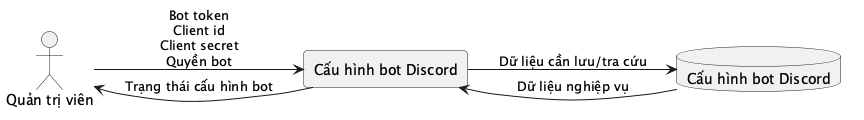
\includegraphics[width=0.95\textwidth,height=0.72\textheight,keepaspectratio]{diagrams/dfd-cau-hinh-bot-discord.png}
    \caption{Sơ đồ luồng dữ liệu: undefined}
\end{figure}

\textbf{Sơ đồ hoạt động}

\begin{figure}[H]
    \centering
    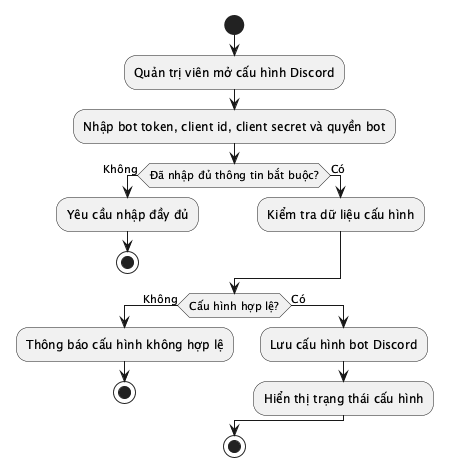
\includegraphics[width=0.95\textwidth,height=0.72\textheight,keepaspectratio]{diagrams/activity-cau-hinh-bot-discord.png}
    \caption{Sơ đồ hoạt động: undefined}
\end{figure}






\subsubsection{Uỷ quyền quản lý Discord Guild}

\textbf{Tóm tắt:} Học sinh ủy quyền Discord để hệ thống có thể quản lý tư cách thành viên Discord Guild của lớp.

\textbf{Tác nhân:} Học sinh, Discord

\textbf{Tiền điều kiện}
\begin{itemize}[leftmargin=*]
    \item Học sinh tồn tại trong hệ thống.
    \item Bot Discord đã được cấu hình.
\end{itemize}

\textbf{Dòng sự kiện chính}
\begin{enumerate}[leftmargin=*]
    \item Học sinh mở đường dẫn ủy quyền Discord.
    \item Hệ thống chuyển học sinh sang trang Discord OAuth.
    \item Học sinh đồng ý cấp quyền identify và guilds.join.
    \item Discord trả mã xác thực về hệ thống.
    \item Hệ thống đổi mã lấy token và lấy thông tin Discord của học sinh.
    \item Hệ thống lưu định danh và token Discord của học sinh.
\end{enumerate}

\textbf{Dòng sự kiện phụ}
\begin{itemize}[leftmargin=*]
    \item Nếu học sinh hủy ủy quyền, hệ thống ghi nhận trạng thái hủy.
    \item Nếu callback thiếu thông tin hoặc state không hợp lệ, hệ thống từ chối xử lý.
\end{itemize}

\textbf{Hậu điều kiện}
\begin{itemize}[leftmargin=*]
    \item Hệ thống có thông tin Discord cần thiết để thêm học sinh vào Guild lớp.
\end{itemize}

\textbf{Sơ đồ luồng dữ liệu}

\begin{figure}[H]
    \centering
    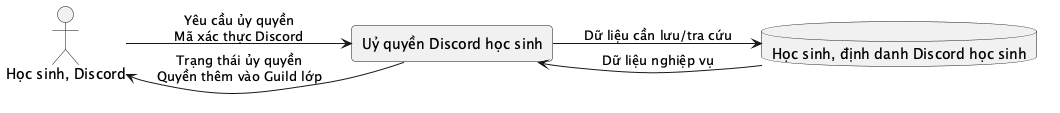
\includegraphics[width=0.95\textwidth,height=0.72\textheight,keepaspectratio]{diagrams/dfd-uy-quyen-discord-guild.png}
    \caption{Sơ đồ luồng dữ liệu: undefined}
\end{figure}

\textbf{Sơ đồ hoạt động}

\begin{figure}[H]
    \centering
    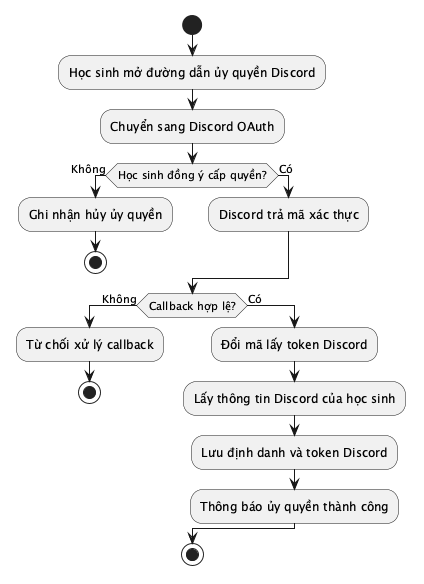
\includegraphics[width=0.95\textwidth,height=0.72\textheight,keepaspectratio]{diagrams/activity-uy-quyen-discord-guild.png}
    \caption{Sơ đồ hoạt động: undefined}
\end{figure}






\subsection{Sơ đồ trạng thái}

State diagram là phần mô hình hóa vòng đời của đối tượng, không phải mô hình
hóa chức năng. Vì vậy phần này chỉ vẽ các đối tượng có trạng thái nghiệp vụ
quan trọng. Việc chọn các đối tượng dưới đây không có nghĩa hệ thống chỉ có các
đối tượng này có trạng thái; các đối tượng khác có thể có status hoặc type
nhưng không đủ phức tạp để cần mô hình trạng thái riêng.

\subsubsection{Trạng thái học sinh}
\begin{figure}[H]
    \centering
    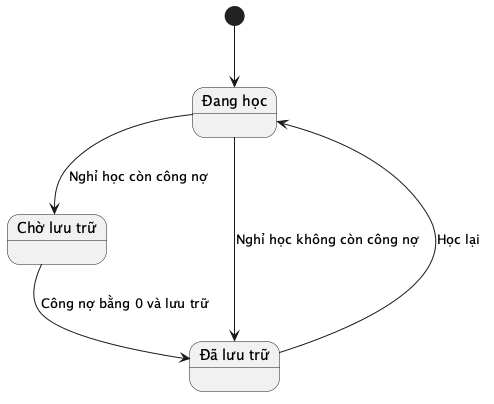
\includegraphics[width=0.95\textwidth,height=0.72\textheight,keepaspectratio]{diagrams/state-hoc-sinh.png}
    \caption{Sơ đồ trạng thái đối tượng Học sinh}
\end{figure}

\subsubsection{Trạng thái buổi học}
\begin{figure}[H]
    \centering
    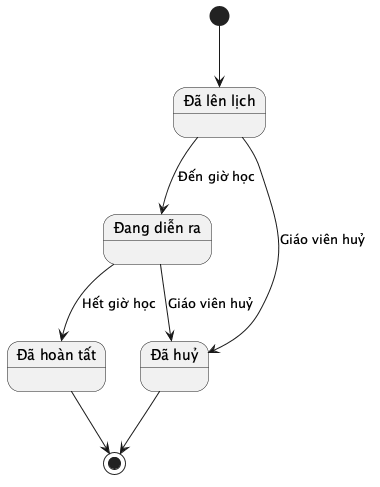
\includegraphics[width=0.95\textwidth,height=0.72\textheight,keepaspectratio]{diagrams/state-buoi-hoc.png}
    \caption{Sơ đồ trạng thái đối tượng Buổi học}
\end{figure}

\end{document}
